\begin{figure}[ht]
	\centering
	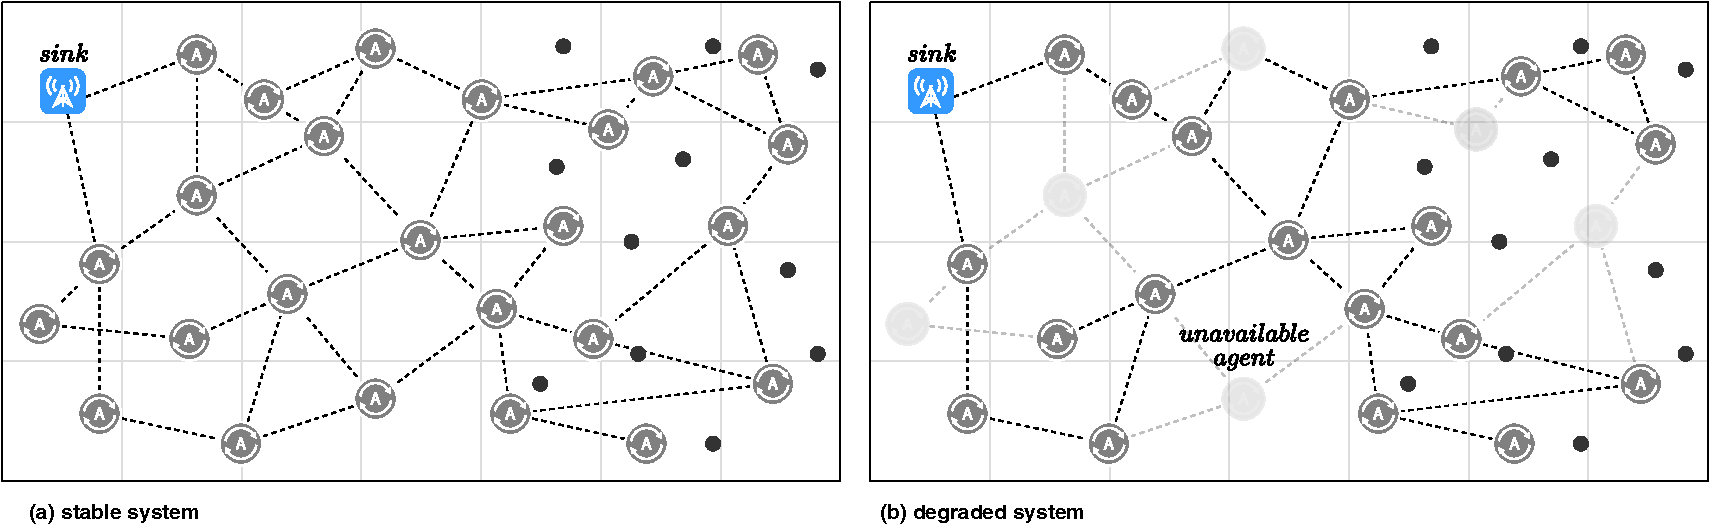
\includegraphics[width=0.9\linewidth]{system-types}
	\caption{\textbf{System types}. The diagram shows examples of the two systems. In the first \simulationSimple{}{}, there are $10$ possible agents that can execute the measurement task, tasks' demand points are distributed across the map. In the second, \simulationExtended{}{} system, there are $25$ agents that can execute the measurement tasks. The tasks' demand points are clustered away from the sink node.}
	\label{fig:system-types}
\end{figure}
\begin{figure}[ht]
	\centering
	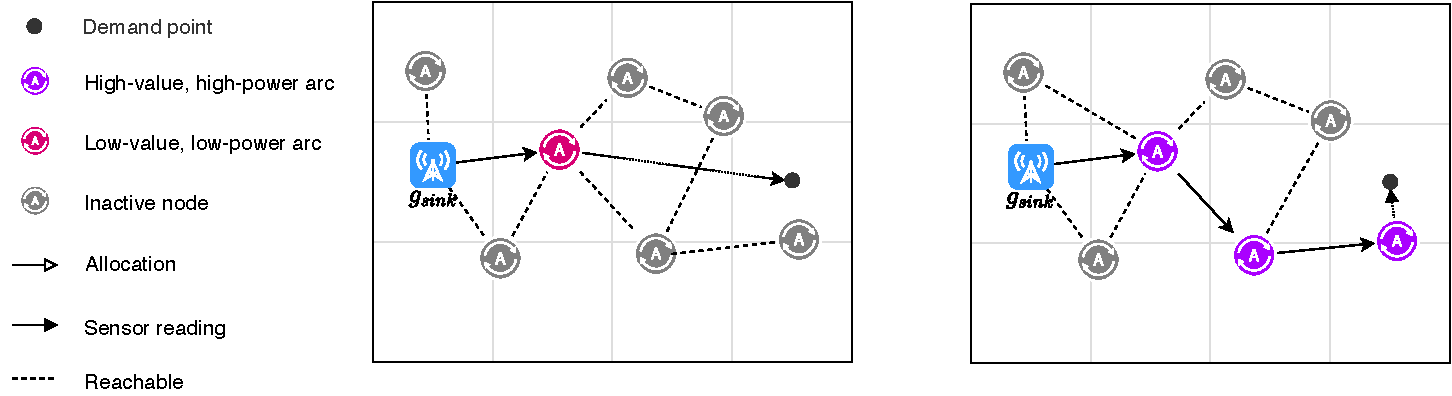
\includegraphics[width=0.9\linewidth]{route-types}
	\caption{\textbf{Routes, power consumption, and task value}. The diagram shows two possible arcs possible for the same system. In the first, energy is conserved by having a short arc but the task is completed to a lesser quality. In the second, the maximum quality for the task is achieved, however, there is more energy consumption overall.}
	\label{fig:route_types}
\end{figure}
We simulated two systems to evaluate the algorithms in four different configurations (See Figure \ref{fig:system-types}).The \simulationSimple{}{} system  equal weighting for each of the CTV components $\alpha, \beta, \gamma$ (Eq. \ref{eq:ctv}). The sink node was given $5$ measurement tasks to complete from outside the system, repeated $3$ times before one episode was complete. $10$ nodes were distributed randomly in the system, each capable of completing a task, or allocating it to any of $3$ nodes it was connected to. Each node could complete any measurement task with a quality dependent on their closeness to the demand point associated with the task (Eq. \ref{eq:atomic_task_quality}). The energy of all nodes in the system was fully reset at the end of each episode. An example of the simple system layout can be seen in Figure \ref{fig:system-types}(a). 

The \simulationExtended{}{} system had CTV component weightings where each of the relevant properties were given an $80\%$ dominance over the value of CTV value. The sink node was given $10$ measurements to allocate, with no repetition. It was also placed at a significantly large distance from the demand points associated with the tasks. $25$ nodes were distributed randomly in the system. This system examined the impact of the algorithm optimising the allocation of tasks towards the goals stated in Section \ref{section:optimisation_problem}. Task value could be maximised, but at the cost of longer arcs and therefore energy usage, or lower task values, and lower energy consumption. Figure \ref{fig:route_types} illustrates these two route types for task completion.

Labels, descriptions, and configurations for each algorithm are shown in Table \ref{table:summary_of_configurations}. Results for the \algorithmBalanced{}{} algorithm in the \simulationSimple{}{} system, and the \algorithmEnergy{}{}, \algorithmQuality{}{}, \algorithmDistribution{}{} algorithms in the \simulationExtended{}{} system are shown in Table \ref{table:results}.

System utility percentages show the summed values of composite tasks per episode, as shown in Equation \ref{eq:system_utility}, compared to the theoretical maximum utility in the system \footnote{Note that the theoretical maximum is not necessarily attainable in all systems, dependent on their randomised node configurations.}, with the percentage optimsations from the first episode to last in Figure \ref{fig:5_ctv-optimal-ctv-gain}. Energy available is presented as a percentage of that of a system containing nodes with full battery charge, see Figure \ref{fig:ctv-statistics-energy-available}. We compare the different biases for optimisation across the CTV components using quality-energy balance, task distribution, and arc-depth results. The quality-energy data uses the \algorithmEnergy{}{} algorithm as a baseline, and shows the percentage increase or decrease in the average task quality over energy availability components of the CTV equation in Equation \ref{eq:ctv}, this is shown in Figure \ref{fig:ctv-quality-energy-baseline-comparison}. Task-distribution, Figure \ref{fig:ctv-task-distribution-comparison},  shows the variation in the agents completing tasks, i.e. $\funcSize{set(\setAgents{}{})}{}/\funcSize{\setAgents{}{}}{}$, with higher values representing more tasks being completed by distinct agents, and lower values meaning more agents are completing multiple tasks. Arc depth data in Figure \ref{fig:ctv-arc-depth-comparison} captures how many nodes re-allocated each task before completion.